\chapter{Making BeagleSNES Portable}

\section{Overview}\index{Overview}

With the small physical size and flexibility of the BeagleBone family of boards, it is natural to consider using BeagleSNES as the software to drive a portable video game system.  To this end, some research has gone into developing such a system and has resulted in the new LCD3 cape display target for BeagleSNES. A prototype portable unit is shown in Figure~\ref{fig:full_unit}.
 
\begin{figure}[h]
\centering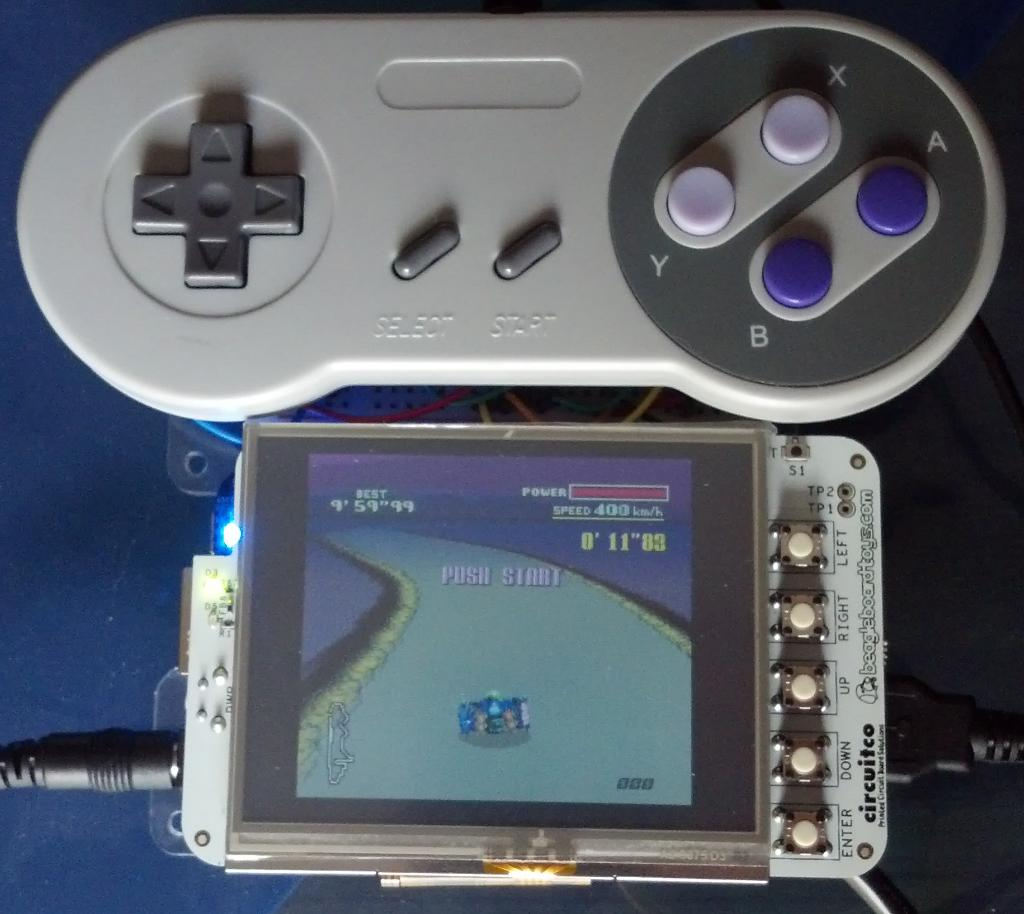
\includegraphics[scale=0.32,clip=true,trim=0 0 0 0]{portable_chapter/full_unit.jpg} 
\caption{A prototype of a portable BeagleSNES system. This prototype still requires a USB gamepad and power via the +5VDC barrel connector, so it isn't fully "portable".}\label{fig:full_unit}
\end{figure}

This target varies from the existing BBB target in the following ways:
\begin{itemize}
\item The LCD3 cape has a resolution of 320x240.  This requires a rework of the BeagleSNES front-end GUI.  On the bright side, such a small resolution allows the emulator to render at the native 256x239 SNES resolution without requiring the use of a software-based pixel-doubler to scale the SNES video output to the higher-resolutions used by the BBB and BB-xM.
\item Additional audio hardware is needed.  For the BBB HDMI target, a dummy CODEC in the kernel provides an ALSA interface to userspace.  Audio data written to the dummy CODEC is passed to the HDMI framer chip in I2S format.  The framer then packages up the audio data and sends it to the display via the HDMI protocol.  When not using the HDMI framer chip, a different audio device must be provided.
\end{itemize}

\section{Video}\index{Video}

The LCD3 cape, seen in Figure~\ref{fig:LCD3}, provides the video display functionality for a portable target.  It weighs approximately 70 grams and has a current consumption of 100mA.  While it is possible to use a smaller display, or at least a display module that has a smaller footprint, the easy availability and pre-packaged nature of the LCD3 cape makes it appealing for quick prototyping without having to worry about device drivers.  

\begin{figure}[h]
\centering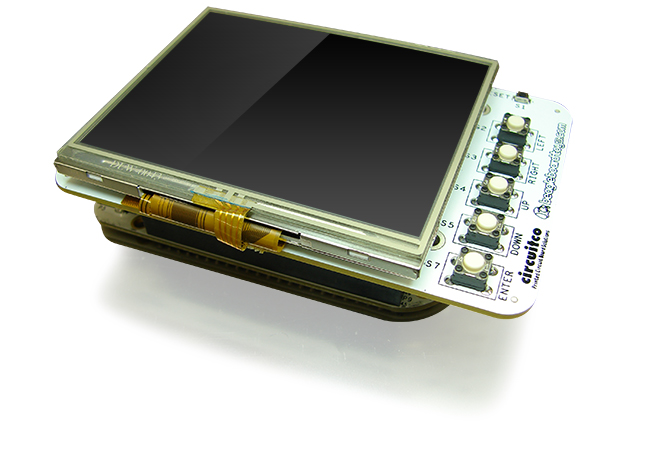
\includegraphics[scale=0.35,clip=true,trim=30 125 30 0]{portable_chapter/LCD3-Front.jpg} 
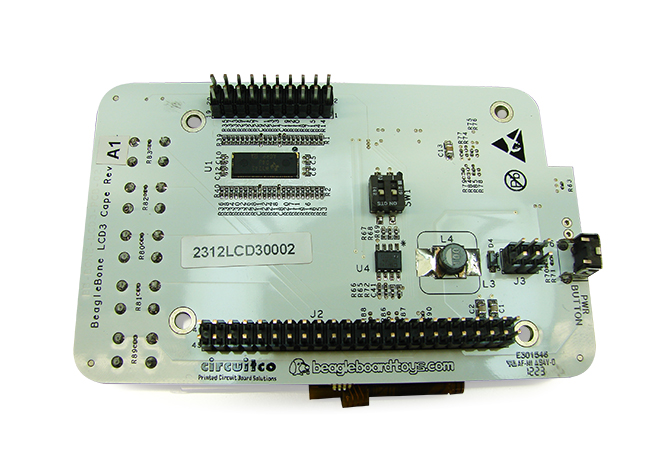
\includegraphics[scale=0.3,clip=true,trim=10 20 15 27]{portable_chapter/LCD3-Bottom.jpg} 
\caption{The LCD3 cape board made by CircuitCo. This 320x240 LCD has a touchscreen and five input buttons (left), and it plugs into the BBB's P8/P9 connectors via pins on the underside of the cape board (right). Photo credit: \texttt{http://elinux.org/CircuitCo:BeagleBone\_LCD3}}\label{fig:LCD3}
\end{figure}

Because the LCD3 cape is defined in the default Device Tree for the BeagleSNES kernel, it will be automatically detected and configured when it is connected to the BBB. The LCD3 uses the \texttt{TILCDC} driver in the kernel to provide a 16 BPP data bus between the BBB and the LCD3 cape.  This is the same driver that is used to communicate with the built-in HDMI cape of the BBB, so userspace software need not be aware of the differences between communicating with the LCD3 cape versus communicating with the HDMI framer chip on the HDMI cape.  As long as the 320x240 resolution is configured as a valid framebuffer resolution (by adding the appropriate framebuffer mode to the \texttt{/etc/fb.modes} file), BeagleSNES can simply request a 320x240 resolution and then adjust its rendering accordingly to use the LCD3 cape.   

\ignore{BeagleSNES makes use of the input features of the LCD3 cape.  The touchscreen is used to adjust the volume of the unit.  Touching the left side of the display will decrease the volume and touching the right side will increase it.  Overlay bars will appear to let you know what the current volume level is whenever the volume has been changed, but they will disappear once there have been no changes in volume change within the last X seconds.  The input buttons on the side of the display are mapped to the up/down/left/right directional pad of the first gamepad, so the game selection GUI can be navigated by using them.  These input features are intended to serve as an implementation reference for anyone wishing to use BeagleSNES to learn and to extend their own work in portable system design.}

\section{Audio}\index{Audio}

The simplest solution for adding audio hardware to the prototype is to use a USB sound device. Such devices are inexpensive (usually around 5-10 USD), quite small (as seen in Figure~\ref{fig:usb_sound}), and readily supported via the USB sound device driver in the kernel.  The configuration to enable this audio driver in the kernel is seen in Figure~\ref{fig:kconfig_audio}.

\begin{figure}[h]
\centering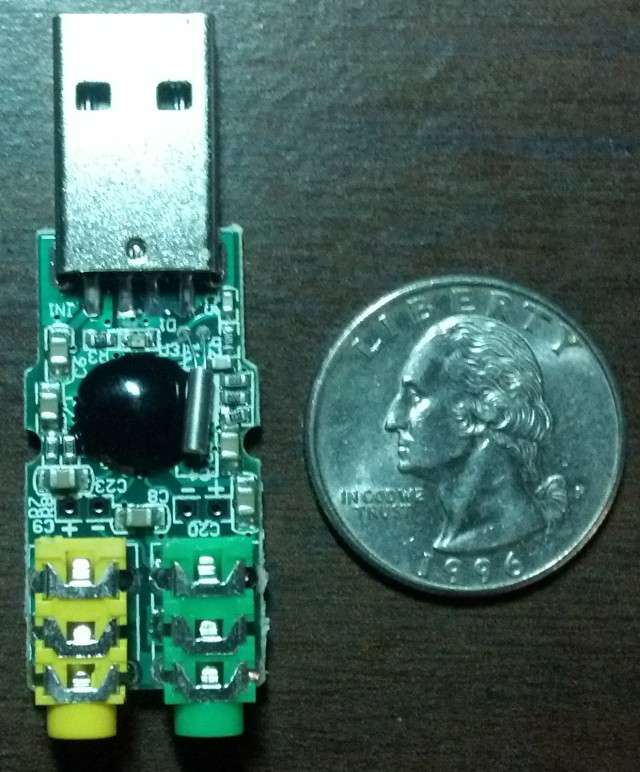
\includegraphics[scale=0.25,clip=true,trim=0 0 0 0]{portable_chapter/usb_sound_quarter.jpg} 
\caption{A USB audio device with its casing removed.}\label{fig:usb_sound}
\end{figure}

\begin{figure}[h]
\begin{verbatim}Device Drivers  --->
   <*> Sound card support  --->
      <*> Advanced Linux Sound Architecture  --->
         [*] USB sound devices  --->
            [*] USB Audio/MIDI driver\end{verbatim}
\caption{The hierarchy within the 3.8 Linux kernel \texttt{kconfig} configuration utility for enabling the USB audio device driver.  BeagleSNES now enables this driver in its BBB kernel for both HDMI and LCD3 video output.}\label{fig:kconfig_audio}
\end{figure}

The BBB only has a single USB port available.  Plugging the USB audio device into it is convenient from an implementation standpoint, but it is inconvenient because the device will extended beyond the footprint of the BBB and LCD3 cape.  Worse yet, a USB port is still needed for the USB gamepad. To resolve these issues, a small, 4-port USB hub is plugged into the single USB port and then used to provide USB to the gamepad and USB audio device.  The hub, when its casing was removed, is so small that it fits into the space between the LCD3 cape and BBB when the cape is plugged into the BBB.

Figure~\ref{fig:usb_hub} shows the positioning of the USB hub and the USB audio device when both components are positioned on top of the BBB.  The USB audio device is soldered directly to one port of the USB hub, allowing the audio jacks to be positioned in a convenient location that isn't limited by the physical position of the USB ports on the hub.  Both the hub and audio device are wrapped in electrical tape to avoid shorting and inadvertent electrical connections.  Because the LCD3 cape only uses a portion of the pins on the P8 connector, the audio jacks are positioned on the connector, next to the ethernet jack.  The assembled unit with all components is shown in Figure~\ref{fig:end_images}.

\begin{figure}[h]
\centering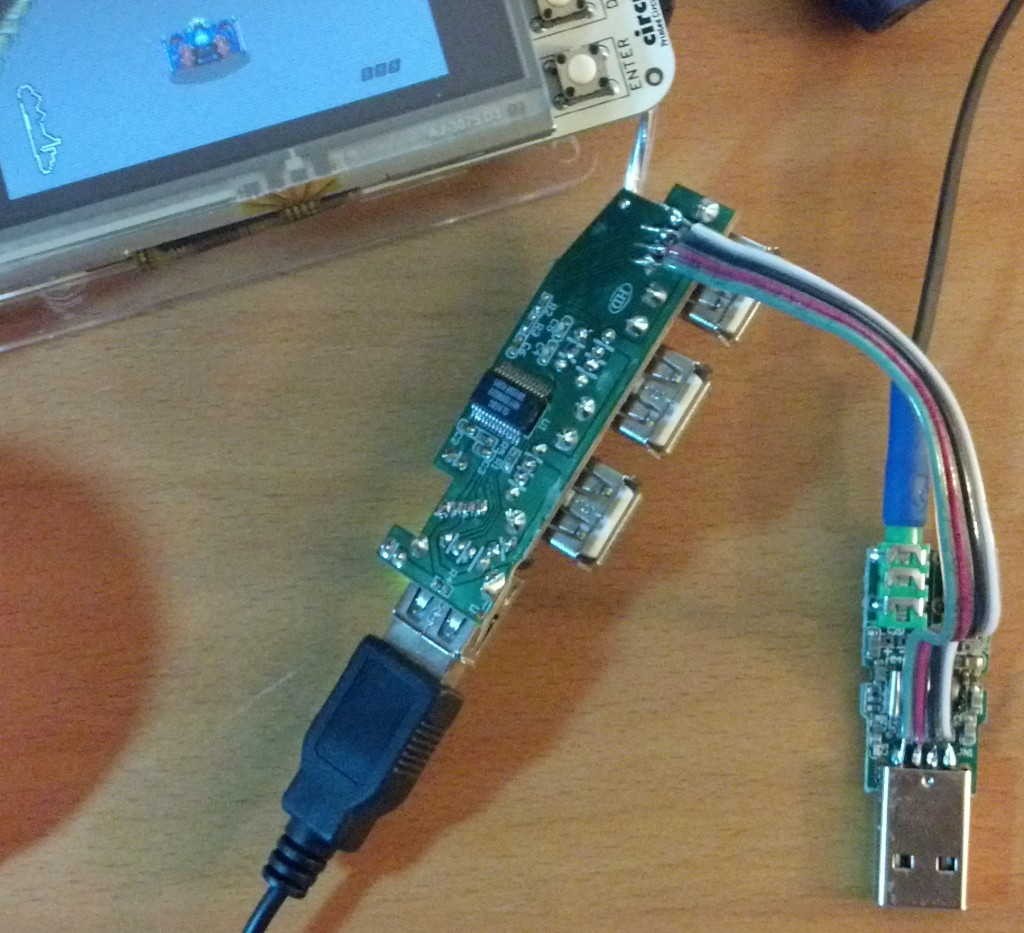
\includegraphics[scale=0.150,clip=true,trim=150 0 0 30]{portable_chapter/usb_hub_solder.jpg} 
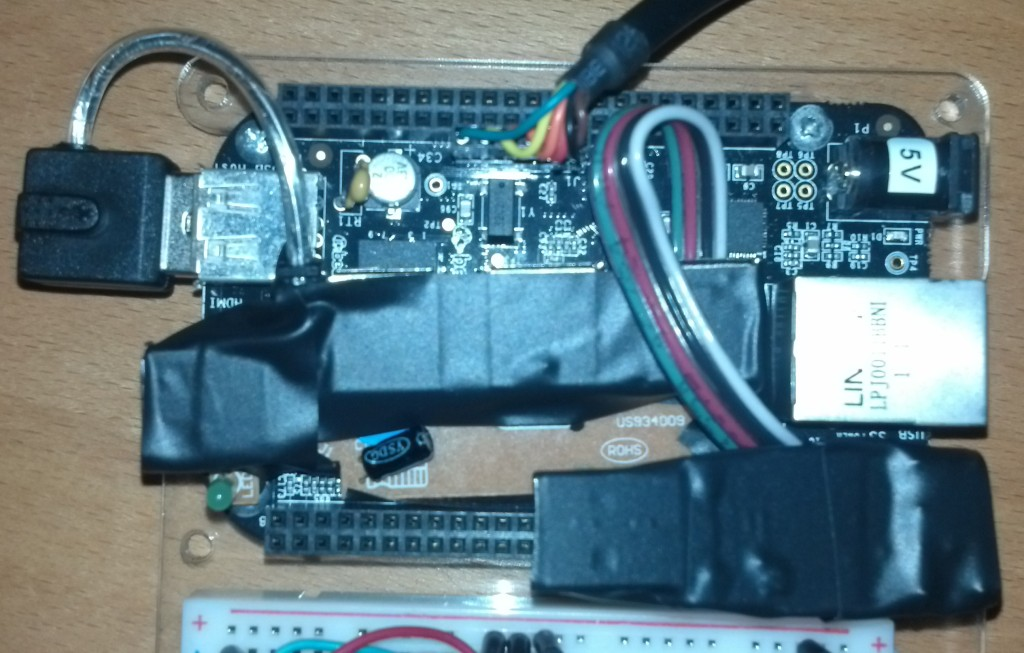
\includegraphics[scale=0.22,clip=true,trim=0 10 0 20]{portable_chapter/half_unit_tape.jpg} 
\caption{The USB hub and audio device. The audio device is soldered directly to a USB port on the hub (left).  Both the hub and device are wrapped in electrical tape and positioned on the BBB.}\label{fig:usb_hub}
\end{figure}

\begin{figure}[h]
\centering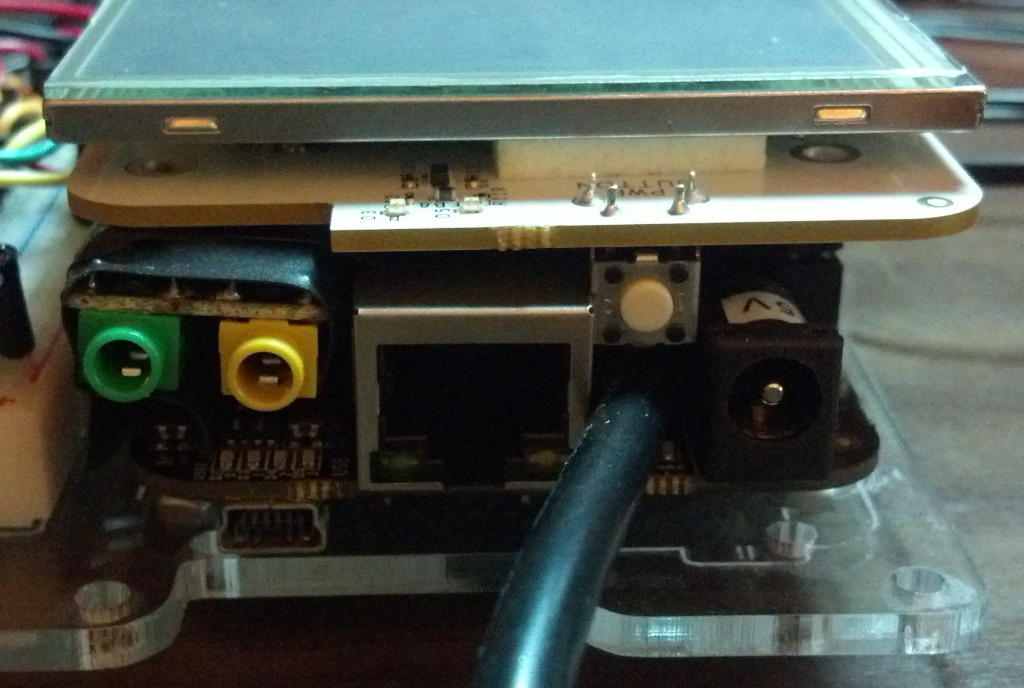
\includegraphics[scale=0.20,clip=true,trim=30 125 30 55]{portable_chapter/edge_power.jpg} 
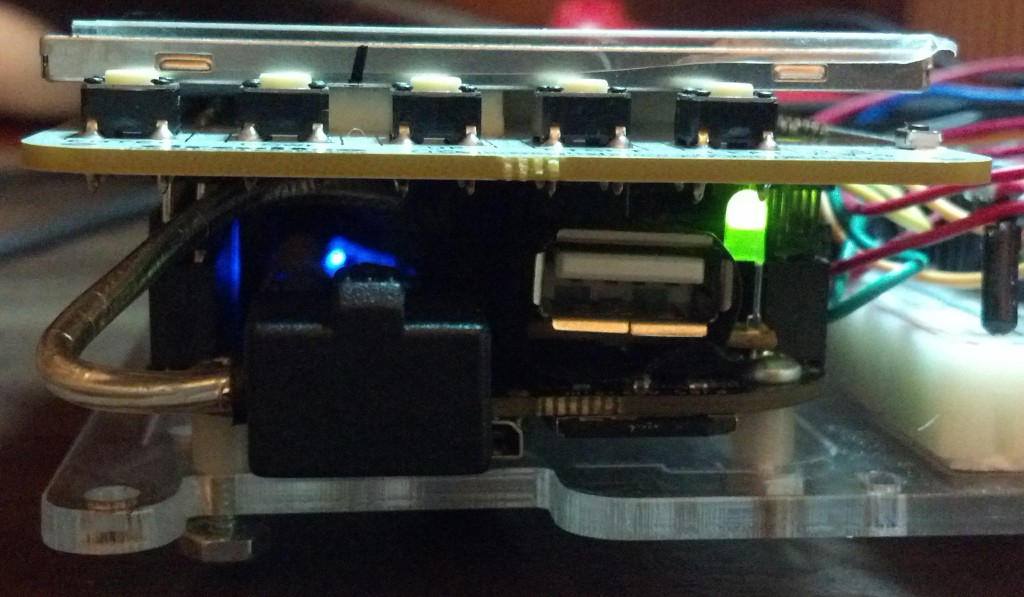
\includegraphics[scale=0.218,clip=true,trim=10 100 20 27]{portable_chapter/edge_usb.jpg} 
\caption{The assembled prototype. The edge of the unit with the power connector (left) exposes the audio jacks and the FTDI debug cable.  The edge of the unit with the BBB USB port (right) exposes the edge of the USB hub and the USB port exposed by the hub. The slight ``tilt'' of the LCD3 cape is due to the height of the FTDI debug cable preventing one side of the cape from being completely inserted.}\label{fig:end_images}
\end{figure}

\begin{updateWarn}
The CircuitCo Audio Cape requires the use of GPIO3[19], which is also used by the LCD3 cape.  So, as the moment, there is no way of using the two together.  A copy of the device tree overlay for the audio cape has been added to \texttt{/lib/firmware} so that you can experiment with the audio cape, but it won't just ``plug-and-play'' like most capes will.  You will have to manually load the overlay for the audio cape to use it.
\end{updateWarn}

\section{GPIO Input}\index{GPIO Input}\label{sec:gpio_hardware}

While requiring the user to use a USB gamepad for input is convenient for the developer, it isn't convenient for the user.  A proper implementation of a portable unit would use GPIO buttons for input and eliminate the need for the USB hub completely.  Luckily, BeagleSNES supports GPIO input.  This allows for a more elegant design for a portable platform, since a custom controller can now be built around the LCD and BBB to minimize the unit's size and weight.

By default, the GPIO support for BeagleSNES on the BBB uses all of the 13 pins on P8.7 through P8.19.  These pins are configured as input pins, and the \texttt{games.xml} file maps these pins to SNES controller events (see Section~\ref{sec:config_gpio}).  In addition, pin P8.2 is used as a ground, and pin P9.3 is used to provide 3.3V. When 3.3V is applied to a GPIO pin, a key down event is placed into the internal application event queue.  When the GPIO pin goes to ground, a key up event is triggered in the same fashion. Figure~\ref{fig:gpio_proto} shows an example implementation of GPIO input for BeagleSNES.  Each pin has a 10k ohm resistor in a pull-down configuration.

 \begin{figure}[h]
\centering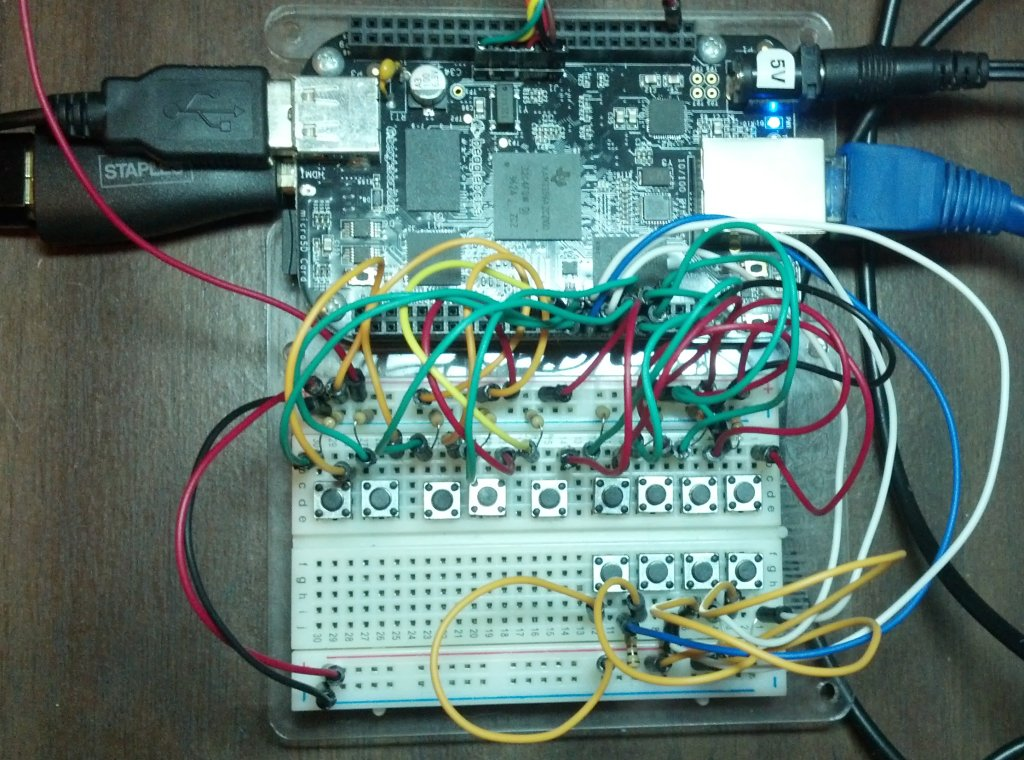
\includegraphics[angle=90,scale=0.22,clip=true,trim=50 20 0 100]{portable_chapter/gpio_proto.jpg}
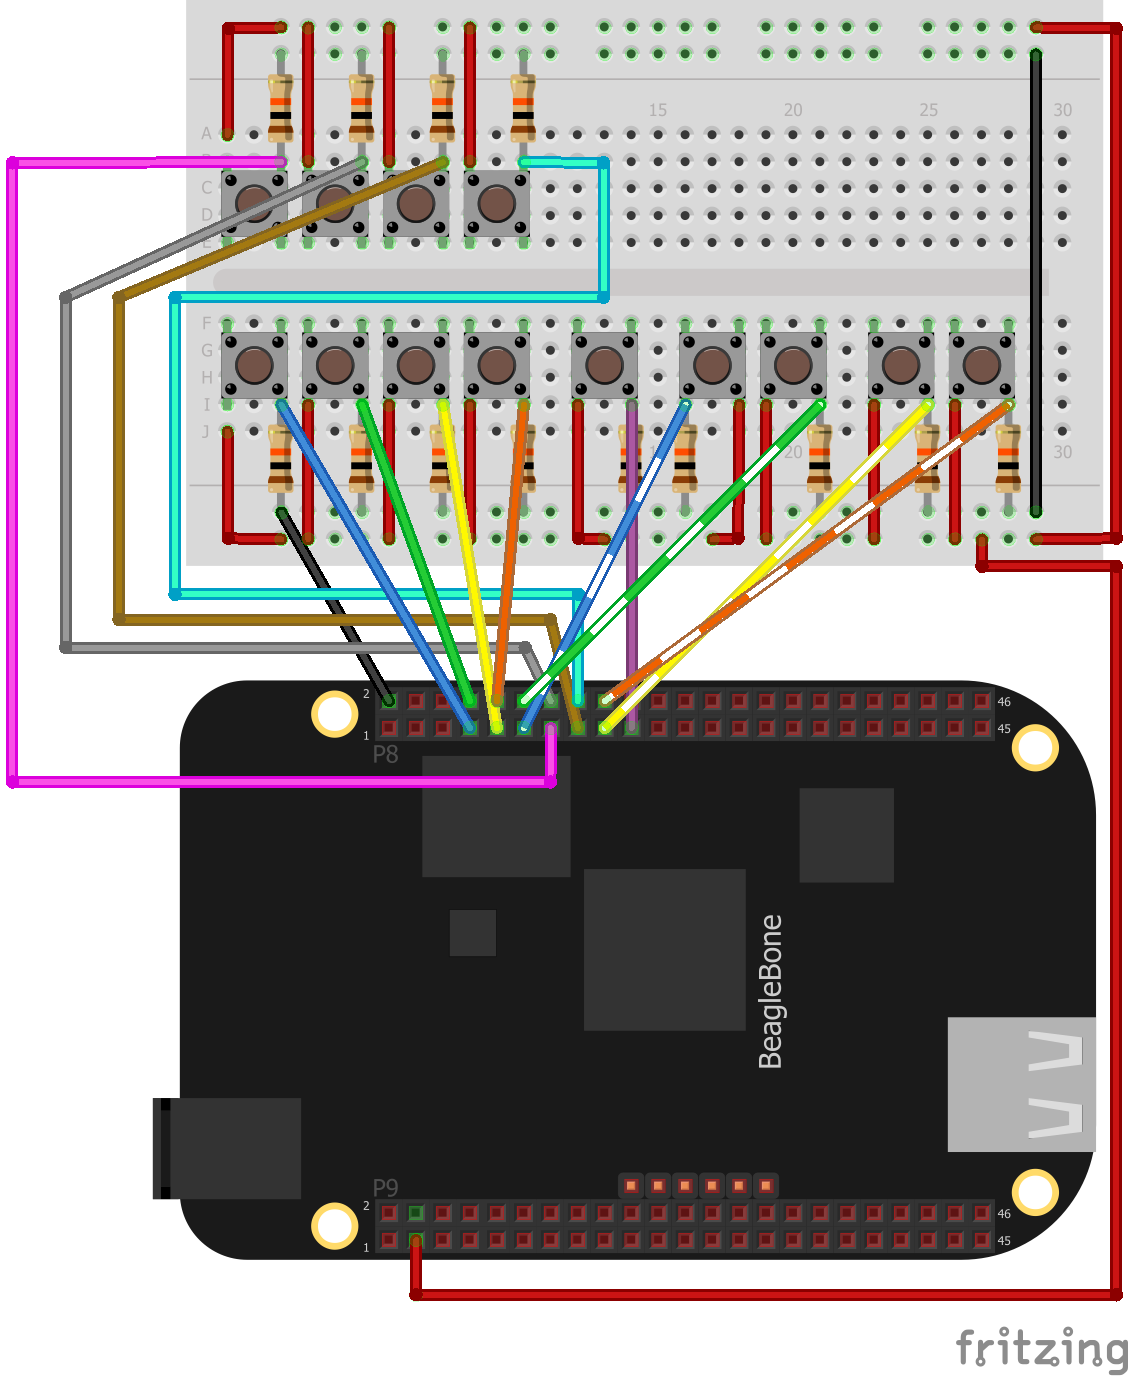
\includegraphics[scale=0.60,clip=true,trim=0 20 0 0]{portable_chapter/GPIO_bb.png}
\caption{Input via GPIO. Thirteen pins are in use in the contiguous block from P8.7 through P8.19. Each pin uses a pull-down resistor configuration. These pins implement the directional pad (4), A/B/X/Y/L/R buttons (6), start/select buttons (2), and a pause button.}\label{fig:gpio_proto}
\end{figure} 

While most of these pins can be easily accessed while the LCD3 cape is attached, pin P9.3 is used to supply power to the LCD3.  To connect to this pin, either put an intermediary ``prototyping'' cape in place that will give you access to the pin or snap a connector onto the P9.3 pin of the LCD3 cape to make a connection.  The prototype in Figure~\ref{fig:gpio_proto} used a logic analyzer probe connector to grab onto the P9.3 pin of the LCD3 cape.

\begin{updateWarn}
Always be very, very careful when working with pins on the BBB that supply voltage.  While pins P9.3 and P9.4 supply 3.3V, pins P9.5 and P9.6 supply 5V.  Connecting a 5V line to a GPIO is a sure-fire way to ruin your BBB, so always exercise caution!
\end{updateWarn}

\section{Other Considerations}\index{Other Considerations}

While the prototype is a good start, there is still work to be done in making a true "portable" system:
\begin{itemize}
\item Power is a consideration.  How much battery life will you get if the emulator is maxing out the CPU?  You'll still need a 5VDC, 2A power supply to power the board with the AM3359 running at maximum capacity.  How heavy will this battery be?  The design of the (now discontinued) CircuitCo battery cape\footnote{\texttt{http://elinux.org/CircuitCo:BeagleBone\_Battery}} might be a good reference point to start designing from.
\end{itemize}
Ultimately, it will come down to how fancy you wish to make your portable unit design and how much money you'd like to spend prototyping it.  The sky is the limit!